
\IEEEPARstart
{I}{n} the first iteration of the design\dots

\subsection{Architecture}
Architecture text here.
\subsection{Hardware}
Current sinknig and sourcing etc. text here.
\subsection{Realization}
    \begin{figure}[h]
        \centering
        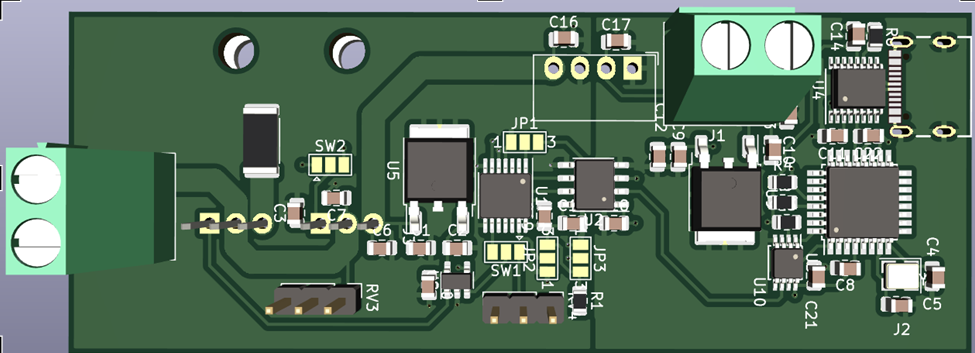
\includegraphics[scale=0.45]{pcb_1st_iteration.png}
        \caption{PCB layout of the 1st iteration of the emulator.}
    \end{figure}


In order to make the first iteration cycle quicker and focus on the modular design 
iteration, the team included a singel cell only in the first PCB. The Fontys laser
printer laboratory was used for the production of the first PCB, however, the via pressing
equipment in the laboratory was incomplete, resulting in a fauty connections. This 
deemed the first PCB unusable, therefore the focus was immediately shifted on the 
second iteration, where the PCB would be ordered and made externally.

\subsection{Testing}
Testing text here.